\documentclass[11pt]{article}

\PassOptionsToPackage{dvipsnames,svgnames,x11names}{xcolor}

% Fonts
\usepackage[osf]{mathpazo}

% BibLaTeX
\usepackage[%
  bibstyle=publist,%
  fixyear=false,%                 Don't print year at very beginning
  hlyear=false,%                  Don't highlight the year
  labeldateparts=false,%          Remove extra 'a', 'b', etc. on year
  % marginyear=true,%
  plnumbering=local-descending,%  Order by most recent
  plauthorhandling=omit,%         Don't print author name
  linktitles=all,%                Add links to all titles
  % authordate,%
  eprint=false,%
  doi=false,%
  url=false,%
  isbn=false,%
  backend=biber%
]{biblatex}
% \addbibresource{bibdatabase.bib}
\addbibresource{bibdatabase-helm.bib}

% Customize bibliography printing
% \AtEveryBibitem{\clearfield{month}}               % Don't use month field
% \AtEveryBibitem{\clearfield{day}}                 % Don't use day field
\DeclareFieldFormat{labelnumberwidth}{#1\adddot}  % Set numbering style

% Page geometry
\usepackage[% iPad
  paperwidth=190.5mm,%
  paperheight=271.88mm,%
  width=136.95mm,%
  height=221.09mm,%
  headsep=1pc,%
  centering,%
]{geometry}
% \usepackage[% standard letter
%   margin=1.25in%
% ]{geometry}

\input{standard-preamble}% Should be loaded late (includes hyperref package)

\definecolor{myblue}{rgb}{0, 0, .75}

\hypersetup{
  colorlinks=true,
  linkcolor={Maroon},
  filecolor={Maroon},
  citecolor={myblue},
  urlcolor={myblue},
}

% Define command for links within bib entries
\ProvideDocumentCommand\link{m}{%
  \href{#1}{\textbf{\small{Preprint.}}}%
}

% Throw away entries of various types that have `notincv` field set to `true`. FIXME: These entry types
% should be listed in the `\defbibfilter`, below!
\DeclareSourcemap{
  \maps[datatype=bibtex]{
    \map{
      \step[fieldsource=notincv,matchi={true},final]% For any entry that has notincv field = true ...
      \step[typesource=article,typetarget=customa]% Change entry type to customa (which gets ignored)
      \step[typesource=incollection,typetarget=customa]
      \step[typesource=online,typetarget=customa]
      \step[typesource=book,typetarget=customa]
      \step[typesource=thesis,typetarget=customa]
      \step[typesource=misc,typetarget=customa]
    }
  }
}

% Print keywords at end of entry, but before abstract and download link.
\ProvideDocumentCommand\categories{m}{#1}
\ProvideDocumentCommand\categoryname{m}{#1}
\NewBibliographyString{keyword,keywords}
\DefineBibliographyStrings{english}{%
  keyword  = {Category},
  keywords = {Categories},
}
\newcounter{cbx@keyword@total}
\newcounter{cbx@keyword@count}
\newcommand*{\keywordscount}[1]{%
\stepcounter{cbx@keyword@total}}
\newcommand*{\keywordsprint}[1]{%
  \stepcounter{cbx@keyword@count}%
  \ifnumless{\value{cbx@keyword@count}}{2}
    {}
    {\addcomma\space}%
    #1%
  }
  % Use categories
  \DeclareFieldFormat{keywords}{%
    \setcounter{cbx@keyword@total}{0}%
    \setcounter{cbx@keyword@count}{0}%
    \forcsvlist{\keywordscount}{#1}%
    % Print "\emph{Categories:} "
    \emph{%
      \categoryname{%
        \ifnumgreater{\value{cbx@keyword@total}}{1}%
          {\bibstring{keywords}}%
          {\bibstring{keyword}}%
          \addcolon%
        }%
      }%
      \space
      % Print list of categories for given entry
      \categories{%
        \forcsvlist{\keywordsprint}{#1}%
      }%
    }%

% Use `download` field in .bib file, and have that linked here to `usera` (default custom field)
\DeclareSourcemap{
  \maps[datatype=bibtex]{
    \map{
      \step[fieldsource=download,fieldtarget=usera]
    }
  }
}
\DeclareFieldFormat{usera}{\link{#1}}
\DeclareFieldFormat{pubstate}{\MakeSentenceCase{#1}}

% Print keywords and download (usera) at end of entry
\renewbibmacro*{addendum+pubstate}{%
  \printfield{addendum}%
  \newunit\newblock
  \printfield{pubstate}%
  \newunit\newblock
  \printfield{keywords}
  \newunit\newblock
  \printfield{usera}
}

% Define htmlabstract environment -- gets redefined in ./webpage-create.cfg
\NewDocumentEnvironment{htmlabstract}{}%
  {\par\begin{small}\textbf{Abstract:}}%
  {\end{small}}

% Print abstract field after bibliography entry
\DeclareFieldFormat{abstract}{#1}
\renewbibmacro*{finentry}{%
  \iffieldundef{abstract}%
  {}%
  {\finentrypunct{} \begin{htmlabstract}\printfield{abstract}\end{htmlabstract}}
  \finentry
}

% Limit TOC to sections and above
\setcounter{tocdepth}{1}

% No title for tableofcontents or bibliography sections
\renewcommand{\contentsname}{}

\newcommand{\onrequest}{\href{mailto:bhelm@fandm.edu}{on request}}

\begin{document}

% Compile this file to .pdf. To generate the .html file, run:
%     execute "source" fnameescape(expand("%:h:~:.")) . "/webpage-create.vim | ToHtml"

\ifx\HCode\undefined
  \title{Webpage}
  \author{Bennett W. Helm\footnote{Department of Philosophy, Franklin \& Marshall College, Lancaster, PA 17601. email: \href{mailto:bennett.helm@fandm.edu}{bennett.helm@fandm.edu}.}}
  \date{}
  \maketitle
\fi

\tableofcontents

\ifdefined\HCode
  \NewLogicalBlock{document}
  \SetTag{document}{div}
  \SetBlockProperty{document}{class}{w3-container}
  \SetBlockProperty{document}{style}{margin-top:15ex;}

  \BlockElementStart{document}{}
\fi

\section[About]{}

\begin{center}
  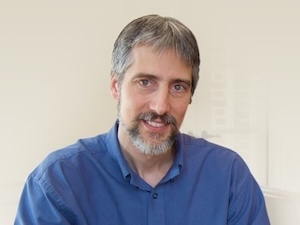
\includegraphics{Helm.jpg}
\end{center}

I am a professor of \href{https://www.fandm.edu/fields-of-study/philosophy/index.html}{philosophy} at \href{https://www.fandm.edu}{Franklin \& {} Marshall College}, and teach courses that are mostly oriented to our \href{https://www.fandm.edu/fields-of-study/cognitive-science/index.html}{Cognitive Science} and \href{https://www.fandm.edu/fields-of-study/moral-psychology/index.html}{Moral Psychology} majors. My research focuses on understanding what it is to be a person as a distinctive sort of free and responsible social agent. Central to my approach is a concern with the \enquote{evaluative attitudes}---caring, valuing, loving, respecting, etc.---and the holistic rational patterns of emotions in terms of which they are intelligible.

\noindent\textbf{Areas of Specialization:}
Moral Psychology and Value Theory,
Philosophy of Emotions,
Social Ontology,
Philosophy of Mind,
Philosophy of Action

\noindent\textbf{Areas of Competence:}
Philosophy of Race and Gender

\subsection*{Academic Positions}

\begin{itemize}
  \item 2013--: Elijah E. Kresge Professor of Philosophy, Franklin \& {} Marshall College
  \item 2007--13: Professor, Franklin \& {} Marshall College
  \item 2001--07: Associate Professor, Franklin \& {} Marshall College
  \item 1995--2001: Assistant Professor, Franklin \& {} Marshall College
\end{itemize}

\subsection*{Education}

\begin{itemize}
  \item PhD in Philosophy, University of Pittsburgh, 1994
  \item MA in Philosophy, University of Pittsburgh, 1990
  \item BA in Philosophy, Carleton College, 1988
\end{itemize}

\noindent\href{https://drive.google.com/file/d/1-8fjo2F9EzgfDyYo_WSTYhaU-xrDNU8P/view}{\textbf{Curriculum Vitae}}.

\section[Research]{Research Overview}

My research aims to understand what it is to be a person, integrating the practical and theoretical dimensions of persons and grounding all of this in an account of the nature of rationality; in this, I weave together moral psychology, value theory, social ontology, philosophy of mind and emotions, and philosophy of action.

Understanding what it is to be a person, I argue, requires understanding various \emph{evaluative attitudes} like caring, valuing, loving, and respecting, and consequently the corresponding kinds of \emph{import} things can have for us. I present an account of such attitudes\slash import fundamentally in terms of the emotions and a distinctively emotional form of rationality, which I call the \enquote{\emph{rationality of import}}. I conclude, first, that the rationality of import has an ineliminably \emph{social} dimension that makes intelligible both (a) our intimate relationships with others and the possibility of our jointly exercising autonomy with them over a shared life, and (b) our constructing what I call \enquote{\emph{communities of respect}}, communities within which alone our capacity for responsible agency can be developed and sustained. Second, I conclude that it is a mistake to conceive of us persons as divided into distinct theoretical and practical sides or to approach understanding personhood via distinct metaphysical and moral notions. Rather, the rationality of import grounds both theoretical and practical rationality. Thus, our theoretical capacity to investigate the world is intelligible as such only together with our practical capacity within communities of respect collectively to value (and hold each other responsible to) public, objective truth. Conversely, our practical capacity to be motivated by value is a kind of responsiveness to value that cannot neatly be separated from our theoretical capacity to contest and ultimately to discover what has such value. Third and finally, this all puts me in a position to argue that we can rationally contest our social identities in a way that makes our social constructions themselves be \emph{objective} insofar as how we construct things can itself be answerable to those very identities as we experience them. And this leads me to the conclusion that we ourselves construct our capacity for autonomous, rational, and responsible agency via the interpersonal and emotional commitments to import we collectively undertake. \emph{Through our practical-cum-theoretical agency, we jointly construct ourselves as persons in a way that is simultaneously answerable to the phenomena of personhood itself.}

I have arrived at these conclusions thus far over the course of three books and work that will become a fourth book, all of which form a single, integrated line of thought taking me from a consideration of (1) \emph{intra}personal values and identity, to (2) \emph{inter}personal values in intimate relationships, to (3) communal norms and values in the context of non-intimate \enquote{communities of respect}, and subsequently to my current research into the objectivity of social identities and ultimately of moral value.

\paragraph{\emph{Emotional Reason} (CUP, 2001).}

One characteristic of us persons is that we value things as a part of the kind of life we each find worth living, thereby partially constituting our identities as the particular persons we are, such that part of our autonomy consists in our ability to determine what our values shall be. On the other hand, we persons can also rationally deliberate about what really is valuable in our lives, thereby potentially coming to discover who we are. Yet such autonomous invention and rational discovery of personal values might seem to be in tension with one another (how can personal values be something we simultaneously both invent and discover?), and this book aims to resolve that tension by developing an account of the relation between emotions and value (or of \enquote{\emph{import}} more generally) that enables me to reject the rational and ontological priority implicit in this formulation of the tension.

In developing this account, I focus not on particular kinds of emotions but rather on the sorts of \emph{rational patterns} emotions can form, arguing that such patterns constitute what it is for things to have import to one. The kind of rationality involved in these patterns of emotions is what I call a \enquote{\emph{rationality of import}}, and it does not fit neatly into standard ways of thinking about practical or theoretical rationality. If we accept (as I do) the Davidsonian thesis that mental capacities are to be understood in terms of an explanatory framework structured by rationality, such a rethinking of rationality means reconceiving the nature of the mind quite generally and of believing and desiring in particular. This enables me to make sense of the distinctive rational role emotions play both in relation to desire and evaluative judgment, thereby dissolving the above tension, and in relation to motivation, thereby making intelligible how we can have rational control over what we do and yet be susceptible to even strong forms of weakness of will. Indeed, I argue that this is essential to presenting an account of the mind adequate to a serious moral psychology.

% For an introduction into the issues discussed in this book, see:
% \begin{enumerate}
%   \item \fullcite{Helm2002Felt-Evaluations-Theory}
%   \item \fullcite{Helm2001Emotions-Practical-Reason}
%   \item \fullcite{Helm2000Emotional-Reason-How}
% \end{enumerate}

\paragraph{\emph{Love, Friendship, and the Self} (OUP, 2010).}

We persons are social animals partly insofar as we are able to form intimate, loving relationships with others, such as familial relationships and relationships of friendship. I argue that standard accounts of friendship are often unsatisfactory because they implicitly presuppose various forms of individualism and egocentrism, thereby failing to capture the intuitive \enquote{depth} such relationships can have in virtue of which we can share our lives and our identities with each other. Instead, I offer an account of love as \emph{intimate identification} in terms of \emph{interpersonal}, rational patterns of emotions. On the one hand this enables me to explain how a caregiver in a loving relationship with a child can provide the child with access to reasons (for being neat or for being moral) that otherwise might seem \enquote{external} to the child's existing motivations. On the other hand, this account enables me to present a rich account of shared agency and ultimately of friendship in terms of the notions of \emph{plural agents} (who not only share certain ends but also the cares motivating those ends) and \emph{plural persons} (who share values and hence a conception of the kind of life worth their living together) and to show how such plural persons can, partly through their rationally intertwined emotions, deliberate together and exercise joint autonomy over their shared lives.

\paragraph{\emph{Communities of Respect} (OUP, 2017).}

To make sense of persons, we must examine as well the \emph{non-intimate} relationships we have with others who are in community with us. In this book I join other Strawsonians in thinking that the reactive attitudes and the ways we \emph{hold} each other responsible are central to our \emph{being} responsible agents at all. Yet in contrast to other accounts, I reject the explanatory priority of the reactive attitudes over our being responsible agents: our reactive attitudes are appropriate in part because they are directed at responsible agents, while simultaneously someone is a responsible agent because they are an appropriate target of the reactive attitudes. I make sense of such circularity as non-vicious by appealing to interpersonal, rational patterns of reactive attitudes, which I argue constitute the community itself, communal norms and values as \emph{our} norms and values, and so individual members of the community as bound by those norms and as having the authority to hold each other responsible to them. Consequently, we in the community \emph{collectively} respect each other as members, and each as one of us ought therefore to respect the others as members. Such an account is not second-personal but \emph{first-person plural}, a conclusion that has several important implications for the social dimension of us persons. First, \emph{responsibility is social}: to be a responsible agent requires that one have the capacity for reactive attitudes, a capacity that one can develop and sustain only as a member of a community of respect. Second, \emph{rationality has a social dimension}: insofar as it is we collectively who have authority over ourselves, we must reject a Humean conception of practical reason (as depending on one's \enquote{subjective motivation set}, say) and recognize an essentially social dimension to practical reason and the possible connections and conflicts among such social reasons and individual reasons grounded in, for example, personal values. Finally, \emph{identity is social}: a community of respect can shape and define certain social identities by prescribing or proscribing communal values as elements of the kind of life worth its members living.

\subsubsection*{}% Empty section to break collapsed paragraph category

\noindent\textbf{Recent Work.}
In the last few years I have begun work on a fourth book that applies these ideas to the nature of social roles and identities, which I understand to be constructed partly through communal norms and values within communities of respect. Social roles and identities presuppose an at least rough-and-ready practical-cum-theoretical understanding in virtue of which such communal norms and values hang together as a coherent whole that can have a point in our lives. Indeed, these understandings must normally come to inform the interpersonal patterns of participants' reactive attitudes that constitute those norms and values and hence the social role or identity itself. This makes room for the possibility that participants' experiences of themselves as occupants of these roles and identities is inconsistent with that understanding and point, providing empirical purchase for rationally contesting those understandings and hence the roles and identities themselves. Whereas other philosophers conceive of such contestation as grounded in unjust \emph{consequences} of these social roles, my claim is that our construction of social roles and identities \emph{itself} can \emph{also} be objective in that our activities of construction, through our holding each other responsible for getting these things right, can come to be answerable to the very roles and identities they thereby construct.

\bigskip{}

Ultimately my aim is to provide an account of moral values as the communal values of the community of respect of all persons, a community in which these values and our personhood itself are both socially constructed yet nonetheless objective.

% \section{Publications}

\section[Books]{Publications: Books}

\newrefsection

\begin{center}
  Links to preprints are to the first chapter.\\
  Full PDFs of final books are available \onrequest{}.\\
  ~
\end{center}

% Cite just things I've written, so that I can filter out only the books
\nocite{Helm2017Communities-Respect-Persons,Helm2010Love-Friendship-Self,Helm2001Emotional-Reason-Deliberation}

\printbibliography[heading=none]

\section[Articles]{Publications: Articles}

\newrefsection
% Now cite everything
\nocite{*}

% FIXME: These entry types should be listed the `\DeclareSourcemap` above!
\defbibfilter{myarticle}{type=article or type=incollection or type=online}

\begin{center}
  PDFs of final articles available \onrequest{}.\\
  ~
\end{center}

Choose a category below.

\printbibliography[filter=myarticle, heading=none]

% \section{Talks}

% \defbibfilter{mytalk}{type=misc}

% \printbibliography[filter=mytalk, heading=none]

\section[Awards]{Fellowships and Awards}

\begin{itemize}
  \item Cowling Distinguished Visiting Professor of Philosophy, Carleton College (2018)
  \item Templeton Foundation Grant (2012--15): \emph{Love and Human Agency: An Interdisciplinary Investigation} (with Agnieszka Jaworska and Jeffrey Seidman), \$640,317
  \item NEH Fellowship (2012--13): \enquote{Defining Moral Communities: Respect, Dignity, and the Reactive Attitudes}, \$50,400
  \item Laurance S. Rockefeller Visiting Faculty Fellow (2012--13), Princeton University Center for Human Values, \$47,000
  \item Bradley R. Dewey Award for Outstanding Scholarship (2012), Franklin \& {} Marshall College
  \item Brocher Foundation Award (2011) for a workshop on \enquote{The Neuroethics of Caring} (with Agnieszka Jaworska), \$36,000
  \item NEH Fellowship (2005--06): \enquote{Love, Friendship and the Self: The Emotional and Interpersonal Grounds of Autonomy}, \$40,000
  \item NSF-CCLI Grant (2001--04): Creation of Artificial Intelligence Laboratory (with Tony Chemero), \$173,281
  \item ACLS Fellowship (1998--99): \enquote{Emotion, Judgment, and Practical Reason: How to Deliberate about Value}, \$20,000
  \item NEH Summer Stipend (1998): \enquote{Reason, Emotion, and Evaluative Judgment: How to Think about the Meaning of Life}, \$6,000
\end{itemize}

\section[Students]{Student Collaborations}

The following is a list of students with whom I've worked on research projects:
\begin{itemize}
  \item Anzhou He (Hackman Scholar, 2023): \enquote{Resisting the Misconstruction of Social Identities: The Interpersonal Call of Ontological Reactive Attitudes}
  \item Raluca Rilla (Hackman Scholar, 2022): \enquote{Objective Self-Constitution of Personhood}
  \item Grace Adams (Hackman Scholar, 2017): \enquote{Race, Gender, and Community}
  \item Dan Kaplan (Hackman Scholar, 2011): \enquote{Joint Caring about Truth}
  \item Kathryn Kutz (Hackman Scholar, 2009): \enquote{Truth, Emotion, and Shared Commitment}
  \item Neal Swisher (Coutros Scholar, 2004): \enquote{Artificial-Life Learning in Mobile Robotics}
  \item Yaroslava Babych and Aleksandra Markovic (Hackman Scholars, 1998), \enquote{Moods as a Sense of Priorities}
\end{itemize}

\section[Courses]{Courses Taught Regularly}

Many of these courses satisfy requirements for our interdisciplinary majors in \href{https://www.fandm.edu/fields-of-study/cognitive-science/index.html}{Cognitive Science} and \href{https://www.fandm.edu/fields-of-study/moral-psychology/index.html}{Moral Psychology}.
\medskip{}

\paragraph{CNX 149: Race, Gender, and Community.}

Race and gender are centrally important to each of our lives. But what are they exactly? How many races or genders are there? Who has what race or what gender? How are these answers determined? (Are race and gender biologically real? Are they socially constructed? Would their being socially constructed make them any less real?) How does someone's race or gender affect their social position? What injustices do these social positions involve, and what can or should we do about them? How are these social positions affected by intersecting social identity categories, including not only race and gender but also class, sexuality, ability, religion, and more? Drawing on fields such as philosophy, sociology, women's and gender studies, and critical race theory, we will critically examine a variety of answers to these questions, in the process trying to understand how we can have reasonable and productive disagreements about these contentious and politically charged issues.

\paragraph{SPM 100: Minds, Machines, and Morals.}

This course provides an introduction to some central problems, concepts, and methods of cognitive science and moral psychology. We will address questions concerning the nature of intelligence, the relationship between minds and bodies, and the basis of moral beliefs and behaviors. These explorations will bridge the sciences and humanities by taking a fundamentally interdisciplinary perspective.

\paragraph{PHI 250: Philosophy of Mind.}

This course is designed as a general introduction to the philosophy of mind (and, consequently, as an introduction to the philosophical side of both majors in the Scientific and Philosophical Studies of Mind program: Cognitive Science and Moral Psychology). We will begin by examining the mind--body problem, a problem which arises out of our differing conceptions of the natural world and of our minds. In particular, science tells us that the body is just a hunk of physical matter that obeys the laws of nature mechanistically---mindlessly. The mind, of course, is anything but mindless. So what's the connection between the two? How should we conceive of the mind in relation to the body? In trying to answer this question, we will critically examine several different purported solutions to this problem and assess how they fare with respect to understanding particular issues that arise in the context of this mind--body problem: the nature of representation, consciousness, psychological explanation, freedom, and meaning, and identity. In addressing these questions, we shall gain a clearer understanding of the strengths, weaknesses, and implications of the various theories about what the mind is and its relation to the body.

\paragraph{PHI 276: Self and Identity.}

Each of us has (is?) a relatively unified self that persists through time and across change. What, then, is a self? What is it for a self at one point in time (as a teenager, for example) to be the same as a self at another point in time (as a grandparent), despite the fact that these selves may in some sense be very different? Traditional philosophical answers have focused rather narrowly on the unity of consciousness and memory. Yet selves include much more than just this: they are defined at least in part by a sense of what is meaningful and important in life, and selves are the sort of thing that can deliberate about meaning and thereby come to take responsibility for themselves. Moreover, selves are in part defined socially, in terms of categories of race and gender, for example. We will explore this richer concept of a self and the implications it has for understanding both who we are at any given moment and our continued identity through time.

\paragraph{PHI 351: Mind-Body Problem.}

It has long been perceived by many philosophers that there is a problem about the relationship between the mind and the body. The body, after all, is just a hunk of physical matter that obeys the laws of nature mechanistically---mindlessly---whereas the mind, of course, is anything but mindless. So what's the connection between the two? How do we conceive of the mind in relation to the body? In this course we'll examine mostly contemporary accounts of the relation in an attempt to understand whether there really is a mind--body problem and, if so, how to solve it. But this course is about more than just the mind and its place in the broader world; it's about the nature of that world, too. In the course of trying to understand how our thoughts can be \emph{about} anything in the world, we'll need to think about the nature of the world such that our thoughts can be about it.

\paragraph{PHI 352: Philosophy of Emotions.}

Long neglected in philosophy, the emotions have recently and increasingly come to be seen as important both in their own right and for their bearing on a wide variety of issues, including (a) the mind--body problem and the nature of consciousness and intentionality, (b) the nature of rationality, (c) aesthetics, (d) interpersonal relationships, and (e) moral psychology and metaethics. My intention in this course is to focus on the first two such issues, since the other issues are covered more fully in other courses. However, in doing so it is important that we have a sufficiently rich understanding of the place emotions can have in our lives, an understanding that many philosophers and psychologists tend to simplify and diminish.

\paragraph{PHI 360: Concept of a Person.}

Philosophers tend to understand the concept of a person in two ways: as a metaphysical notion and as a moral notion. \emph{Moral personhood} is roughly an understanding of ourselves as the subjects of moral rights and responsibilities. By contrast, to understand personhood as a \emph{metaphysical} notion is to understand it as delineating a special category of being---as having or being a soul, for example. Typically, the metaphysical notion of personhood is thought to somehow underwrite our status as moral persons. Indeed, it is precisely because of this explanatory link between them that many philosophers think it is appropriate to understand the concept of personhood not as having two senses but rather as being a univocal concept with two aspects. Our aim in this course is to examine these notions and their interrelations, with an emphasis on our social nature.

\paragraph{PHI 361: Moral Psychology.}

Moral psychology is the study of us persons as responsible moral agents and subjects of value. As such, it is constrained by, and must cohere with, the facts about human psychology; but its primary focus is on human good, an evaluative notion. Topics include virtue and character, motivation and reasons, internal/external reasons and moral development, and responsibility and blame.

\paragraph{PHI 362: Love and Friendship.}

Love and friendship are undoubtedly important in our lives \dots{} but why? Although we commonly say that we \enquote{love} both chocolate cake and philosophy or that we are \enquote{friends} with people on Facebook, these seem to be thin surrogates for the potentially deep, rich, intimate, and rewarding attitudes and relationships we develop towards and with other persons. Clearly it is the latter that we interested in here: forms of love and friendship that apply paradigmatically to intimate relations among persons. In investigating personal love and friendship, we will encounter several problems concerning their justification, their bearing on the autonomy and identity of the individual, and the place their value has within a broader system of values, including moral values.

\paragraph{PHI 363: Respect, Responsibility, and Ethics.}

Recently many philosophers have argued that certain interpersonal emotions, such as resentment, indignation, guilt, gratitude, and approbation, are fundamental to a host of interconnected issues in ethics, including the nature of respect, dignity, responsibility and freedom, and the origins of moral values. This course will closely examine these claims and arguments with the aim of understanding more clearly how moral psychology and metaethics intersect.

\ifdefined\HCode
  \BlockElementEnd{document}
\fi

\end{document}
